\documentclass[aspectratio=169]{beamer}
\setbeamerfont{headline}{size=\footnotesize}

\mode<presentation>{
    \usetheme{Montpellier}
    \setbeamercovered{transparent}
    \usecolortheme{beaver}
}

\usepackage[english,brazil]{babel}
\usepackage[utf8]{inputenc}
\usepackage{fontawesome}
\usepackage{graphicx}
\usepackage{url}
\usepackage{colortbl}
\usepackage{caption}
\usepackage{booktabs}
\usepackage{tikz}
\usetikzlibrary{positioning,arrows.meta,fit,backgrounds,shapes.multipart,
                shapes,arrows,calc,trees}
\usepackage{pgfplots}
\pgfplotsset{compat=1.18}
\usepackage{ragged2e}

% --- Cores ---
\definecolor{mineblue}{RGB}{0,90,180}
\definecolor{mineorange}{RGB}{230,115,0}
\definecolor{minegreen}{RGB}{34,139,34}
\definecolor{minered}{RGB}{180,20,40}
\definecolor{minegray}{RGB}{100,100,100}

% --- Comandos auxiliares ---
\newcommand{\reflexao}[1]{\begin{alertblock}{Reflexão}#1\end{alertblock}}
\newcommand{\key}[1]{\underline{#1}}

% --- Dados do Título ---
\title[Mineração de Dados]{Mineração de Dados: Conceitos e Aplicações}
\subtitle{Módulo 6: Métodos Estatísticos e Clustering}
\author[Elton Sarmanho]{
    Prof. Elton Sarmanho\inst{1}\\
    \footnotesize \href{mailto:eltonss@ufpa.br}{eltonss@ufpa.br}
}
\institute[UFPA]{
    \inst{1} Faculdade de Sistemas de Informação - UFPA Campus Cametá
}
\date{\today}

% --- TikZ estilos ---
\tikzstyle{block} = [rectangle,draw,fill=mineblue!20,text width=5em,
                     text centered,rounded corners,minimum height=3em,
                     font=\small]
\tikzstyle{line}  = [draw,-latex']

\begin{document}

% ==============================================================================
% Título
% ==============================================================================
\begin{frame}
    \titlepage
    \begin{center}
        \tiny \faGithub\ \href{https://github.com/eltonsarmanho}{github.com/eltonsarmanho} \quad
        \faLinkedinSquare\ \href{https://www.linkedin.com/in/elton-sarmanho-836553185/}{Elton Sarmanho}
    \end{center}
\end{frame}

% Roteiro
\begin{frame}[shrink=5]{Roteiro da Aula}
    \tableofcontents
\end{frame}

% ==============================================================================
\section{Fundamentos Estatísticos}
% ==============================================================================

\subsection{Testes de Hipótese}

% --- Frame: O que é Teste de Hipótese ---
\begin{frame}[shrink=8]{O que é um Teste de Hipótese?}
    \begin{columns}
        \column{0.55\textwidth}
        \begin{block}{Definição}
            \footnotesize
            Procedimento para \textbf{decidir}, com base em evidências amostrais, se uma afirmação sobre uma população deve ser aceita ou rejeitada.
        \end{block}
        \begin{block}{Componentes Essenciais}
            \begin{itemize}\footnotesize
                \item \textbf{$H_0$ (hipótese nula):} posição padrão a testar\\
                      ex. ``RF e SVM têm mesma acurácia''
                \item \textbf{$H_1$ (alternativa):} o que queremos provar
                \item \textbf{Nível de significância $\alpha$:} geralmente $0{,}05$
                \item \textbf{p-valor:} rejeita $H_0$ se $p < \alpha$
            \end{itemize}
        \end{block}
        \column{0.45\textwidth}
        \centering
        \begin{tikzpicture}[scale=0.78,font=\tiny,
            box/.style={rectangle,draw=mineblue,fill=mineblue!10,
                        rounded corners,minimum width=2.8cm,
                        minimum height=0.7cm,align=center,font=\small},
            arr/.style={-{Stealth[length=5pt]},mineblue,thick}]
            \node[box] (h)   at (0,0)    {Formular $H_0$, $H_1$};
            \node[box] (d)   at (0,-1.1) {Coletar Dados};
            \node[box] (t)   at (0,-2.2) {Calcular estatística};
            \node[box] (p)   at (0,-3.3) {Calcular p-valor};
            \node[box,fill=minegreen!15,draw=minegreen]
                       (dec) at (0,-4.4) {Decisão: $p < \alpha$?};
            \node[font=\tiny,minered]  (rej) at ( 1.8,-5.2) {Rejeitar $H_0$};
            \node[font=\tiny,minegreen](nrj) at (-1.8,-5.2) {Não rejeitar $H_0$};
            \draw[arr] (h)--(d); \draw[arr] (d)--(t);
            \draw[arr] (t)--(p); \draw[arr] (p)--(dec);
            \draw[arr,minered]   (dec.south east) -- (rej.north);
            \draw[arr,minegreen] (dec.south west) -- (nrj.north);
        \end{tikzpicture}
    \end{columns}
\end{frame}

% --- Frame: Tipos de Erro ---
\begin{frame}[shrink=5]{Tipos de Erro e Poder do Teste}
    \begin{columns}
        \column{0.5\textwidth}
        \begin{block}{Tipos de Erro}
            \begin{center}
            \begin{tabular}{lcc}
            \toprule
            & $H_0$ verdadeira & $H_0$ falsa \\
            \midrule
            Não rejeitar & \textcolor{minegreen}{\faCheck\ Correto} & \textcolor{minered}{Erro Tipo II ($\beta$)} \\
            Rejeitar     & \textcolor{minered}{Erro Tipo I ($\alpha$)} & \textcolor{minegreen}{\faCheck\ Poder ($1-\beta$)} \\
            \bottomrule
            \end{tabular}
            \end{center}
        \end{block}
        \begin{alertblock}{Atenção}
            \footnotesize Reduzir $\alpha$ aumenta $\beta$. Há um \textbf{trade-off} entre os dois tipos de erro. O poder do teste aumenta com maior $n$ (mais dados).
        \end{alertblock}
        \column{0.5\textwidth}
        \begin{block}{Testes Relevantes em Mineração de Dados}
            \begin{itemize}\footnotesize
                \item \textbf{Teste $t$ pareado:} compara 2 classificadores nos mesmos folds
                \item \textbf{ANOVA:} compara 3 ou mais classificadores simultaneamente
                \item \textbf{Wilcoxon Signed-Rank:} alternativa não-paramétrica ao teste $t$
                \item \textbf{McNemar:} compara classificadores pelas matrizes de confusão
            \end{itemize}
        \end{block}
        \vspace{0.1cm}
        \centering\tiny \faArrowRight\ Consulte o Material Didático Módulo 6 para exemplos detalhados
    \end{columns}
\end{frame}

% --- Frame: Teste t Pareado ---
\begin{frame}[shrink=5]{Teste $t$ Pareado: Comparando Dois Algoritmos}
    \begin{columns}
        \column{0.5\textwidth}
        \begin{block}{Fórmula}
            \[
              t = \frac{\bar{d}}{s_d / \sqrt{n}}, \quad
              \bar{d} = \frac{1}{n}\sum_{i=1}^{n}(a_i - b_i)
            \]
        \end{block}
        \begin{block}{Exemplo: RF vs SVM (10 folds)}
            \footnotesize
            $\bar{d} = 2{,}40\%$, $s_d = 0{,}91$, $n=10$
            \[
              t = \frac{2{,}40}{0{,}91/\sqrt{10}} \approx 8{,}33
            \]
            $t_{\text{crítico}}(gl=9, \alpha=0{,}05) = 1{,}833$\\[4pt]
            Como $8{,}33 \gg 1{,}833$: \textbf{rejeitamos $H_0$}\\
            RF é estatisticamente superior ao SVM $(p < 0{,}001)$
        \end{block}
        \column{0.5\textwidth}
        \begin{block}{Quando usar}
            \begin{itemize}\footnotesize
                \item Dois algoritmos avaliados nos \textit{mesmos} folds (amostras pareadas)
                \item Diferenças aproximadamente normais
                \item Para $n < 30$ verificar normalidade das diferenças
            \end{itemize}
        \end{block}
        \begin{alertblock}{Significância $\neq$ Relevância Prática}
            \footnotesize $p < 0{,}05$ indica que a diferença provavelmente não é aleatória, mas $\Delta = 2{,}4\%$ pode ou não ser relevante dependendo do custo do erro na aplicação.
        \end{alertblock}
        \centering\tiny \faArrowRight\ Exemplo completo: Material Didático e Colab Módulo 6
    \end{columns}
\end{frame}

% --- Frame: ANOVA ---
\begin{frame}[shrink=6]{ANOVA: Comparando Três ou Mais Algoritmos}
    \begin{columns}
        \column{0.52\textwidth}
        \begin{block}{Objetivo}
            \footnotesize Comparar \textbf{simultaneamente} $k \geq 3$ algoritmos.\\
            $H_0$: todas as médias são iguais.\\
            $H_1$: pelo menos uma difere.
        \end{block}
        \begin{block}{Exemplo: KNN vs DT vs NaiveBayes}
            \footnotesize
            \begin{center}
            \begin{tabular}{lccc}
            \toprule
            & KNN & DT & NB \\
            \midrule
            Média & 83\% & 79{,}8\% & 75\% \\
            \bottomrule
            \end{tabular}
            \end{center}
            $F = MS_{\text{entre}}/MS_{\text{dentro}} = 81{,}05/2{,}40 \approx 33{,}77$\\
            $F_{\text{crit}}(2,12) = 3{,}89$: \textbf{rejeita $H_0$} $(p < 0{,}001)$
        \end{block}
        \column{0.48\textwidth}
        \begin{alertblock}{Pós-ANOVA}
            \footnotesize ANOVA diz que \textit{alguma} diferença existe, mas não \textit{qual par} difere. Use:
            \begin{itemize}\footnotesize
                \item \textbf{Tukey HSD} ou \textbf{Bonferroni} para comparações de pares
                \item \textbf{Friedman + Nemenyi} para abordagem não-paramétrica em $k$ algoritmos
            \end{itemize}
        \end{alertblock}
        \begin{block}{Wilcoxon Signed-Rank}
            \footnotesize Alternativa ao teste $t$ quando:
            \begin{itemize}\footnotesize
                \item $n < 30$ sem garantia de normalidade
                \item Presença de \textbf{outliers} nos dados
                \item Dados \textbf{ordinais} (scores de ranking)
            \end{itemize}
            Ranqueia $|d_i|$ e testa se a mediana das diferenças é zero.
        \end{block}
    \end{columns}
\end{frame}

% ==============================================================================
\subsection{Correlação e Dependência}
% ==============================================================================

% --- Frame: Pearson ---
\begin{frame}[shrink=8]{Correlação de Pearson}
    \begin{columns}
        \column{0.5\textwidth}
        \begin{block}{Definição}
            \[
              r = \frac{\sum(x_i-\bar{x})(y_i-\bar{y})}
                       {\sqrt{\sum(x_i-\bar{x})^2 \cdot \sum(y_i-\bar{y})^2}}
              \in [-1,1]
            \]
        \end{block}
        \begin{block}{Escala de Interpretação}
            \begin{center}\footnotesize
            \begin{tabular}{cc}
            \toprule
            $|r|$ & Interpretação \\
            \midrule
            $0{,}90$--$1{,}00$ & Muito forte \\
            $0{,}70$--$0{,}89$ & Forte \\
            $0{,}50$--$0{,}69$ & Moderada \\
            $0{,}30$--$0{,}49$ & Fraca \\
            $< 0{,}30$        & Desprezível \\
            \bottomrule
            \end{tabular}
            \end{center}
        \end{block}
        \column{0.5\textwidth}
        \centering
        \begin{tikzpicture}[scale=0.72,font=\tiny]
        \begin{axis}[
            width=7cm, height=5.5cm,
            xlabel={Horas de Estudo},
            ylabel={Nota Final},
            xmin=0.5, xmax=11, ymin=3, ymax=11,
            grid=major, grid style={dotted,gray!40},
            axis lines=left,
            title={\small \textbf{Horas de Estudo vs Nota ($r=0{,}88$)}},
            title style={color=mineblue},
            xlabel style={font=\tiny},
            ylabel style={font=\tiny},
            tick label style={font=\tiny},
        ]
            \addplot[only marks,mark=*,mineblue,mark size=2.5pt,
                     mark options={fill=mineblue}]
              coordinates {(2,4.5)(3,5.0)(4,5.5)(5,6.0)(6,7.5)(7,8.0)(9,9.0)(10,9.5)};
            \addplot[minered,thick,domain=1.5:11,samples=2] {0.605*x+4.2};
            \node[font=\tiny,minered] at (axis cs:7.5,6.3) {tendência};
        \end{axis}
        \end{tikzpicture}
        \begin{alertblock}{}
            \footnotesize \textbf{Correlação $\neq$ Causalidade.} Pearson mede apenas relação \textbf{linear}. Para relações não lineares, use Spearman ou Informação Mútua.
        \end{alertblock}
    \end{columns}
\end{frame}

% --- Frame: Spearman e Informação Mútua ---
\begin{frame}[shrink=6]{Spearman, Kendall e Informação Mútua}
    \begin{columns}
        \column{0.5\textwidth}
        \begin{block}{Correlação de Spearman ($\rho$)}
            \footnotesize
            Aplica Pearson sobre os \textbf{postos} (\textit{ranks}) dos dados.
            \begin{itemize}\footnotesize
                \item Detecta relações \textbf{monotônicas} (não só lineares)
                \item Robusta a outliers
                \item Indicada para dados ordinais ou com distribuição assimétrica
            \end{itemize}
        \end{block}
        \begin{block}{Tau de Kendall ($\tau$)}
            \footnotesize
            Baseado em pares \textbf{concordantes/discordantes}.
            \begin{itemize}\footnotesize
                \item Mais robusto que Spearman para amostras pequenas
                \item Interpretação probabilística direta
            \end{itemize}
        \end{block}
        \column{0.5\textwidth}
        \begin{block}{Informação Mútua $I(X;Y)$}
            \[
              I(X;Y) = \sum_{x,y} p(x,y)\log\frac{p(x,y)}{p(x)\,p(y)}
            \]
            \begin{itemize}\footnotesize
                \item Mede dependência \textbf{geral} (não apenas linear)
                \item $I(X;Y) = 0$ somente se $X$ e $Y$ são independentes
                \item Amplamente usado em \textbf{seleção de features} (MRMR)
                \item Captura relações complexas que Pearson ignora
            \end{itemize}
        \end{block}
        \vspace{0.2cm}
        \centering\tiny \faArrowRight\ Consulte Material Didático para exemplo prático com cálculo de Pearson
    \end{columns}
\end{frame}

% ==============================================================================
\section{Agrupamento (Clustering)}
% ==============================================================================

\subsection{Conceitos Gerais}

% --- Frame: O que é Clustering ---
\begin{frame}[shrink=7]{O que é Clustering?}
    \begin{columns}
        \column{0.52\textwidth}
        \begin{block}{Definição}
            \footnotesize
            Tarefa de \textbf{aprendizado não-supervisionado} que organiza exemplos similares em grupos (clusters) sem o uso de rótulos pré-definidos.
        \end{block}
        \begin{block}{Aplicações}
            \begin{itemize}\footnotesize
                \item \faArrowRight\ \textbf{Segmentação de clientes:} grupos de comportamento de compra
                \item \faArrowRight\ \textbf{Detecção de anomalias:} pontos sem cluster são outliers
                \item \faArrowRight\ \textbf{Compressão de imagens:} quantização de cores com K-Means
                \item \faArrowRight\ \textbf{Bioinformática:} agrupamento de genes por expressão
                \item \faArrowRight\ \textbf{Modelagem de tópicos:} agrupamento de documentos
            \end{itemize}
        \end{block}
        \column{0.48\textwidth}
        \centering
        \begin{tikzpicture}[scale=0.85,font=\tiny]
            % Cluster 1 (azul)
            \foreach \x/\y in {1.0/2.0,1.3/2.5,1.6/1.8,0.8/1.5,1.5/2.8}{
                \fill[mineblue,opacity=0.8] (\x,\y) circle (4pt);
            }
            \draw[mineblue,dashed,thick] (1.2,2.1) circle (0.85);
            \node[mineblue,font=\small\bfseries] at (1.2,0.8) {Cluster 1};
            % Cluster 2 (laranja)
            \foreach \x/\y in {3.5/3.2,3.8/2.8,4.1/3.5,3.3/3.0,4.0/2.5}{
                \fill[mineorange,opacity=0.8] (\x,\y) circle (4pt);
            }
            \draw[mineorange,dashed,thick] (3.7,3.0) circle (0.85);
            \node[mineorange,font=\small\bfseries] at (3.7,1.8) {Cluster 2};
            % Cluster 3 (verde)
            \foreach \x/\y in {2.5/0.5,2.8/0.8,2.2/0.8,2.6/0.2}{
                \fill[minegreen,opacity=0.8] (\x,\y) circle (4pt);
            }
            \draw[minegreen,dashed,thick] (2.5,0.5) circle (0.65);
            \node[minegreen,font=\small\bfseries] at (2.5,1.4) {Cluster 3};
            % Ponto anômalo
            \fill[minered] (0.2,3.8) circle (4pt);
            \node[minered,font=\tiny] at (0.6,4.0) {outlier?};
        \end{tikzpicture}
        \begin{alertblock}{}
            \footnotesize Avalie resultados com métricas \textbf{e} visualização (PCA, t-SNE, UMAP).
        \end{alertblock}
    \end{columns}
\end{frame}

% ==============================================================================
\subsection{K-Means}
% ==============================================================================

% --- Frame: K-Means conceito ---
\begin{frame}[shrink=7]{K-Means: Conceito e Objetivo}
    \begin{columns}
        \column{0.5\textwidth}
        \begin{block}{Objetivo: Minimizar Inércia}
            \[
              J = \sum_{k=1}^{K} \sum_{\mathbf{x}_i \in C_k}
                  \|\mathbf{x}_i - \boldsymbol{\mu}_k\|^2
            \]
            onde $\boldsymbol{\mu}_k$ é o centróide do cluster $k$.
        \end{block}
        \begin{block}{Resumo do Algoritmo (Lloyd, 1982)}
            \begin{enumerate}\footnotesize
                \item Inicializar $K$ centróides (aleatório ou K-Means++)
                \item \textbf{Atribuição:} cada ponto vai ao centróide mais próximo
                \item \textbf{Atualização:} mover centróide para a média do cluster
                \item Repetir 2--3 até convergência
            \end{enumerate}
        \end{block}
        \column{0.5\textwidth}
        \begin{block}{Propriedades}
            \begin{itemize}\footnotesize
                \item \textbf{Complexidade:} $O(n \cdot K \cdot d \cdot i)$, onde $d$ é a dimensão e $i$ o número de iterações
                \item \textbf{Convergência:} garantida (mas pode ser ótimo local)
                \item \textbf{Limitações:} assume clusters \textbf{esféricos e de tamanho similar}; sensível a outliers e inicialização
                \item \textbf{Distância:} euclidiana por padrão
            \end{itemize}
        \end{block}
        \vspace{0.1cm}
        \centering\tiny \faArrowRight\ Consulte Material Didático e Colab para implementação em Python
    \end{columns}
\end{frame}

% --- Frame: K-Means passo a passo ---
\begin{frame}[shrink=12]{K-Means: Passo a Passo com Exemplo}
    \begin{columns}
        \column{0.5\textwidth}
        \begin{block}{Exemplo: $K=2$, ponto $\mathbf{x}=(5,3)$}
            \footnotesize
            Centróides iniciais: $C_1=(2,4)$ e $C_2=(6,1)$\\[4pt]
            \textbf{Passo 3: Atribuição}
            \begin{align*}
              d(\mathbf{x},C_1) &= \sqrt{9+1} \approx 3{,}16 \\
              d(\mathbf{x},C_2) &= \sqrt{1+4} \approx 2{,}24
            \end{align*}
            $\Rightarrow$ atribuir $(5,3)$ ao cluster $C_2$
        \end{block}
        \begin{block}{\small Passo 4: Recalcular centróide}
            \footnotesize
            Pontos em $C_1$: $(3,4),(4,1),(2,3),(2,6),(3,3)$
            \[
              \boldsymbol{\mu}_1 = \tfrac{1}{5}(14,\,17) = (2{,}8,\; 3{,}4)
            \]
        \end{block}
        \column{0.5\textwidth}
        \centering
        \begin{tikzpicture}[scale=0.80,font=\tiny]
            \draw[->,thick,minegray] (0,0)--(7,0) node[right]{$x$};
            \draw[->,thick,minegray] (0,0)--(0,6) node[above]{$y$};
            % Pontos C1 (azul)
            \foreach \x/\y in {3/4,4/1,2/3,2/6,3/3}{
                \fill[mineblue,opacity=0.8] (\x,\y) circle (4pt);
            }
            % Pontos C2 (laranja)
            \fill[mineorange,opacity=0.8] (5,3) circle (4pt)
                node[right,mineorange] {$(5,3)$};
            % Centróides
            \fill[minered] (2,4) circle (5pt)
                node[left,minered] {$C_1$};
            \fill[minered] (6,1) circle (5pt)
                node[right,minered] {$C_2$};
            % Seta distâncias
            \draw[minered,dashed] (5,3)--(2,4)
                node[midway,above,minered] {$3{,}16$};
            \draw[minered,dashed] (5,3)--(6,1)
                node[midway,right,minered] {$2{,}24$};
            % Novo centróide C1
            \fill[minegreen,opacity=0.9] (2.8,3.4) circle (5pt)
                node[right,minegreen] {\textbf{novo} $\mu_1$};
            % legenda
            \fill[mineblue] (0.3,5.5) circle (3pt);
            \node[right,mineblue] at (0.5,5.5) {C1 original};
            \fill[minegreen] (0.3,5.0) circle (3pt);
            \node[right,minegreen] at (0.5,5.0) {C1 atualizado};
            \fill[minered] (0.3,4.5) circle (4pt);
            \node[right,minered] at (0.5,4.5) {centróide};
        \end{tikzpicture}
    \end{columns}
\end{frame}

% --- Frame: Figura K-Means ---
\begin{frame}[shrink=12]{K-Means: Visualização das Etapas}
    \begin{center}
        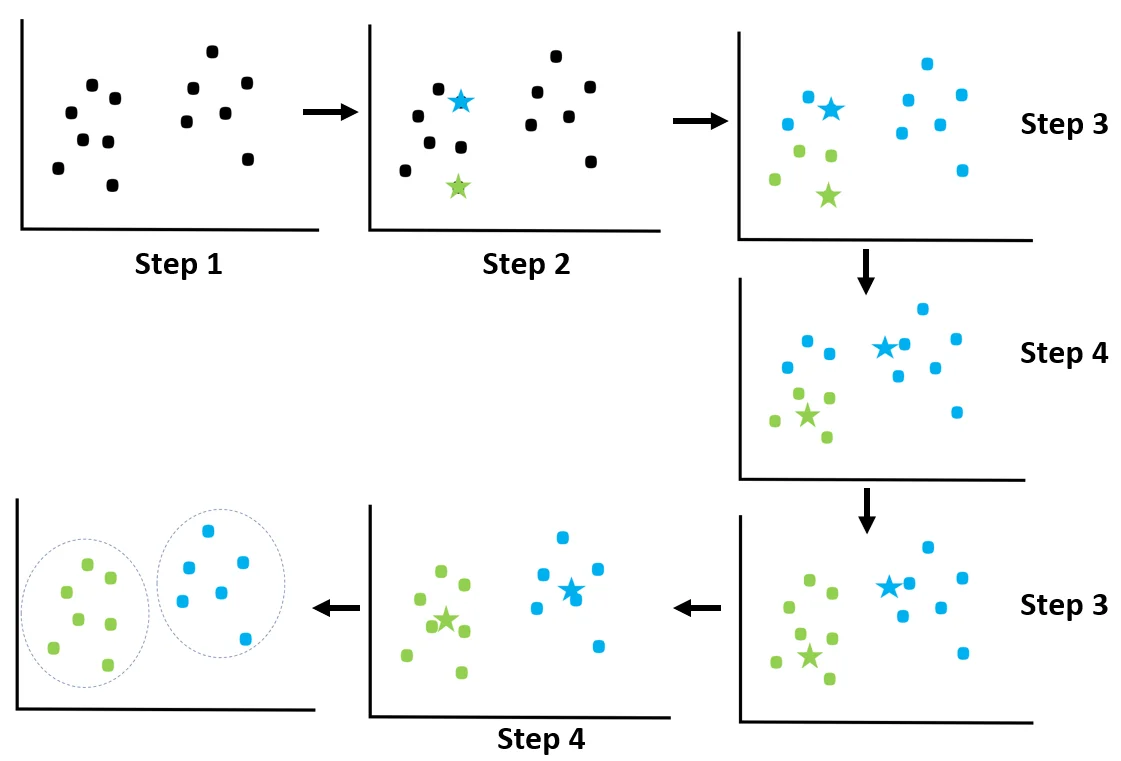
\includegraphics[width=0.7\textwidth]{figs/EtapasKmeans.png}
    \end{center}
    \begin{block}{}
        \centering\footnotesize
        Cada iteração atualiza centróides até que os clusters se estabilizem.\\
        \faArrowRight\ Ver algoritmo completo no Material Didático Módulo 6.
    \end{block}
\end{frame}

% --- Frame: Escolha de K - Elbow ---
\begin{frame}{Escolha de K: Método do Cotovelo}
    \begin{columns}
        \column{0.45\textwidth}
        \begin{block}{Ideia}
            \footnotesize
            Plota a \textbf{inércia} (WCSS) para $K=1,2,\ldots$. O ponto onde a redução desacelera, formando um ``cotovelo'', indica o $K$ ótimo.
            \[
              \text{WCSS}(K) = \sum_{k=1}^{K}\sum_{\mathbf{x}_i \in C_k}\|\mathbf{x}_i-\boldsymbol{\mu}_k\|^2
            \]
        \end{block}
        \begin{alertblock}{Limitação}
            \footnotesize O cotovelo pode ser ambíguo em dados sobrepostos. Combine sempre com a \textbf{Análise de Silhouette}.
        \end{alertblock}
        \column{0.55\textwidth}
        \centering
        \begin{tikzpicture}[scale=0.85]
        \begin{axis}[
            width=8cm, height=5cm,
            xlabel={\small Número de Clusters ($K$)},
            ylabel={\small Inércia (WCSS)},
            xmin=0.5, xmax=6.5, ymin=0, ymax=2600,
            xtick={1,2,3,4,5,6},
            grid=major, grid style={dotted,gray!40},
            axis lines=left,
            title={\small\textbf{Método do Cotovelo}},
            title style={color=mineblue},
            tick label style={font=\tiny},
            xlabel style={font=\small},
            ylabel style={font=\small},
        ]
            \addplot[mineblue,very thick,mark=*,mark size=2.5pt,
                     mark options={fill=mineblue}]
                coordinates {(1,2400)(2,1200)(3,480)(4,420)(5,390)(6,375)};
            \draw[minered,dashed,thick] (axis cs:3,0)--(axis cs:3,480);
            \node[above right,font=\tiny,color=minered] at (axis cs:3,480)
                {$K^*=3$};
            \fill[minered] (axis cs:3,480) circle (3pt);
        \end{axis}
        \end{tikzpicture}
        \vspace{0.1cm}
        \tiny De $K=2$ para $K=3$: queda de $-60\%$ na inércia. De $K=3$ em diante: ganho marginal pequeno.
    \end{columns}
\end{frame}

% --- Frame: Silhouette ---
\begin{frame}[shrink=5]{Escolha de K: Análise de Silhouette}
    \begin{columns}
        \column{0.50\textwidth}
        \begin{block}{Coeficiente de Silhouette}
            \footnotesize
            Para cada ponto $\mathbf{x}_i$ no cluster $C_k$:
            \begin{align*}
              a(i) &= \text{distância média intra-cluster}\\
              b(i) &= \text{distância média ao vizinho mais próximo}
            \end{align*}
            \[
              s(i) = \frac{b(i)-a(i)}{\max\{a(i),b(i)\}} \in [-1,\,1]
            \]
        \end{block}
        \begin{block}{Interpretação}
            \begin{itemize}\footnotesize
                \item $s \approx +1$: ponto bem dentro do cluster
                \item $s \approx 0$: ponto na fronteira
                \item $s \approx -1$: ponto no cluster errado
                \item $\bar{s} > 0{,}5$: clustering de qualidade
            \end{itemize}
        \end{block}
        \column{0.50\textwidth}
        \centering
        \begin{tikzpicture}[scale=0.85]
        \begin{axis}[
            width=7.5cm, height=5cm,
            xlabel={\small Número de Clusters ($K$)},
            ylabel={\small Silhouette Score $\bar{s}$},
            xmin=1.5, xmax=5.5, ymin=0, ymax=0.85,
            xtick={2,3,4,5},
            grid=major, grid style={dotted,gray!40},
            axis lines=left,
            title={\small\textbf{Silhouette Score por $K$}},
            title style={color=mineblue},
            tick label style={font=\tiny},
            xlabel style={font=\small},
            ylabel style={font=\small},
        ]
            \addplot[minegreen,very thick,mark=square*,mark size=2.5pt,
                     mark options={fill=minegreen}]
                coordinates {(2,0.71)(3,0.58)(4,0.42)(5,0.29)};
            \draw[minered,dashed,thick] (axis cs:2,0)--(axis cs:2,0.71);
            \node[above right,font=\tiny,color=minered] at (axis cs:2,0.71)
                {$K^*=2$};
            \fill[minered] (axis cs:2,0.71) circle (3pt);
        \end{axis}
        \end{tikzpicture}
        \begin{alertblock}{}
            \footnotesize Use \textbf{Elbow} e \textbf{Silhouette} juntos para maior confiabilidade na escolha de $K$.
        \end{alertblock}
    \end{columns}
\end{frame}

% --- Frame: Variantes K-Means ---
\begin{frame}[shrink=5]{Variantes do K-Means}
    \begin{columns}
        \column{0.5\textwidth}
        \begin{block}{K-Means++}
            \footnotesize
            Inicialização inteligente: cada centróide é escolhido com probabilidade proporcional à distância ao centróide mais próximo já escolhido.
            \begin{itemize}\footnotesize
                \item Evita inicializações ruins
                \item Garante aproximação $O(\log K)$ do ótimo
                \item \textbf{Padrão} no scikit-learn
            \end{itemize}
        \end{block}
        \begin{block}{K-Medoids (PAM)}
            \footnotesize
            Usa exemplos reais como centróides (medóides).
            \begin{itemize}\footnotesize
                \item Mais robusto a outliers que K-Means
                \item Interpretável: centróide é um ponto real
                \item Mais custoso computacionalmente
            \end{itemize}
        \end{block}
        \column{0.5\textwidth}
        \begin{block}{Mini-Batch K-Means}
            \footnotesize
            Atualiza centróides com mini-lotes aleatórios a cada iteração.
            \begin{itemize}\footnotesize
                \item Escala para datasets de \textbf{milhões} de exemplos
                \item Resultado ligeiramente pior que K-Means padrão
                \item Ideal para dados em stream
            \end{itemize}
        \end{block}
        \begin{alertblock}{Quando K-Means falha}
            \footnotesize Clusters não esféricos, de tamanhos muito diferentes, ou com muitos outliers. Nesses casos, prefira DBSCAN, GMM ou Spectral Clustering.
        \end{alertblock}
    \end{columns}
\end{frame}

% ==============================================================================
\subsection{Clustering Hierárquico}
% ==============================================================================

% --- Frame: Clustering Hierárquico ---
\begin{frame}[shrink=12]{Clustering Hierárquico}
    \begin{columns}
        \column{0.50\textwidth}
        \begin{block}{Conceito}
            \footnotesize
            Cria uma \textbf{hierarquia} de agrupamentos em um \textbf{dendrograma}, sem necessitar especificar $K$ antecipadamente.
        \end{block}
        \begin{block}{Abordagens}
            \begin{itemize}\footnotesize
                \item \textbf{Agglomerativo (bottom-up):} começa com $N$ clusters e mescla os dois mais próximos iterativamente
                \item \textbf{Divisivo (top-down):} começa com um cluster e divide recursivamente
            \end{itemize}
        \end{block}
        \begin{block}{Critérios de Ligação}
            \begin{itemize}\footnotesize
                \item \textbf{Single:} distância mínima, sensível a outliers
                \item \textbf{Complete:} distância máxima, clusters compactos
                \item \textbf{Average (UPGMA):} equilíbrio entre os dois
                \item \textbf{Ward:} minimiza variância intra-cluster (mais popular)
            \end{itemize}
        \end{block}
        \column{0.50\textwidth}
        \centering
        \begin{tikzpicture}[scale=0.85,
            level 1/.style={sibling distance=3.5cm,level distance=1.6cm},
            level 2/.style={sibling distance=1.7cm,level distance=1.4cm},
            level 3/.style={sibling distance=0.9cm,level distance=1.1cm},
            edge from parent/.style={draw,mineblue,thick}]
        \node[draw=mineblue,fill=mineblue!10,rounded corners,
              font=\small\bfseries] {Raiz}
          child { node[draw=mineorange,fill=mineorange!10,
                       rounded corners,font=\small] {A}
            child { node[draw=minegreen,fill=minegreen!10,
                         rounded corners,font=\tiny] {A1}
              child { node[font=\tiny] {$p_1$} }
              child { node[font=\tiny] {$p_2$} }
            }
            child { node[draw=minegreen,fill=minegreen!10,
                         rounded corners,font=\tiny] {A2}
              child { node[font=\tiny] {$p_3$} }
              child { node[font=\tiny] {$p_4$} }
            }
          }
          child { node[draw=mineorange,fill=mineorange!10,
                       rounded corners,font=\small] {B}
            child { node[font=\tiny] {$p_5$} }
            child { node[draw=minegreen,fill=minegreen!10,
                         rounded corners,font=\tiny] {B2}
              child { node[font=\tiny] {$p_6$} }
              child { node[font=\tiny] {$p_7$} }
            }
          };
        \end{tikzpicture}
        \vspace{0.1cm}
        \tiny Cortar o dendrograma em diferentes alturas define diferentes números de clusters.
    \end{columns}
\end{frame}

% ==============================================================================
\subsection{DBSCAN e HDBSCAN}
% ==============================================================================

% --- Frame: DBSCAN ---
\begin{frame}[shrink=5]{DBSCAN: Clustering Baseado em Densidade}
    \begin{columns}
        \column{0.5\textwidth}
        \begin{block}{Conceito}
            \footnotesize
            Encontra clusters de \textbf{forma arbitrária} e detecta \textbf{ruído/outliers} automaticamente. Parâmetros: $\varepsilon$ (raio) e MinPts (vizinhos mínimos).
        \end{block}
        \begin{block}{Tipos de Pontos}
            \begin{itemize}\footnotesize
                \item \textcolor{mineblue}{\textbf{Núcleo:}} $\geq$ MinPts vizinhos em raio $\varepsilon$
                \item \textcolor{minegreen}{\textbf{Fronteira:}} dentro do raio de um núcleo, mas não é núcleo
                \item \textcolor{minered}{\textbf{Ruído:}} não é núcleo nem fronteira
            \end{itemize}
        \end{block}
        \begin{alertblock}{Vantagem sobre K-Means}
            \footnotesize Não precisa especificar $K$. Detecta clusters de qualquer forma geométrica e identifica outliers automaticamente.
        \end{alertblock}
        \column{0.5\textwidth}
        \centering
        \begin{tikzpicture}[scale=0.95,font=\tiny]
            % Cluster 1 (azul)
            \foreach \x/\y in {1.5/1.0,2.0/1.5,1.0/1.5,2.5/1.0,
                                1.8/2.0,1.2/0.8,2.2/0.8,2.8/1.5}{
                \filldraw[mineblue!50] (\x,\y) circle(0.07);
            }
            \draw[mineblue,dashed,thick] (1.8,1.4) circle(0.75);
            \filldraw[mineblue] (1.8,1.4) circle(0.09);
            \node[above=0.8cm,mineblue,font=\tiny] at (1.8,1.4)
                {núcleo ($\varepsilon$)};
            % Cluster 2 (laranja)
            \foreach \x/\y in {4.0/3.0,4.5/3.5,5.0/3.0,4.8/2.5,3.8/2.8,5.2/3.5}{
                \filldraw[mineorange!60] (\x,\y) circle(0.07);
            }
            % Fronteira
            \filldraw[minegreen,thick] (3.2,2.0) circle(0.09)
                node[right,minegreen] {\;fronteira};
            % Ruído
            \filldraw[minered] (6.3,1.0) circle(0.09)
                node[right,minered] {\;ruído};
            \filldraw[minered] (0.3,3.6) circle(0.09)
                node[right,minered] {\;ruído};
            \node[below,font=\tiny,minegray] at (3.2,0.2)
                {Clusters: azul e laranja | ruído: vermelho};
        \end{tikzpicture}
        \vspace{0.1cm}
        \tiny Estimar $\varepsilon$ pelo gráfico da $k$-NN distance (joelho da curva).
    \end{columns}
\end{frame}

% --- Frame: HDBSCAN ---
\begin{frame}{HDBSCAN: Extensão Hierárquica do DBSCAN}
    \begin{columns}
        \column{0.5\textwidth}
        \begin{block}{Limitação do DBSCAN}
            \footnotesize
            DBSCAN usa um único $\varepsilon$ global. Se os clusters têm \textbf{densidades diferentes}, um único limiar não funciona bem.
        \end{block}
        \begin{block}{HDBSCAN (McInnes et al., 2017)}
            \footnotesize
            Varia o limiar de densidade automaticamente ao longo de uma hierarquia. Extrai os clusters mais \textbf{persistentes}.
            \begin{itemize}\footnotesize
                \item Apenas \texttt{min\_cluster\_size} é crítico
                \item Detecta clusters com densidades variáveis
                \item Retorna \textbf{probabilidade} de pertencimento
                \item Padrão no scikit-learn $\geq$ 1.3
            \end{itemize}
        \end{block}
        \column{0.5\textwidth}
        \begin{block}{Pipeline UMAP + HDBSCAN}
            \footnotesize
            Abordagem moderna para dados de alta dimensão:
            \begin{center}
            \begin{tikzpicture}[scale=0.85,font=\small,
                box/.style={rectangle,draw=mineblue,fill=mineblue!10,
                            rounded corners,minimum width=2.5cm,
                            minimum height=0.65cm,align=center},
                arr/.style={-{Stealth[length=4pt]},mineblue,thick}]
                \node[box] (raw)   at (0,0)    {Dados (alta dim.)};
                \node[box] (umap)  at (0,-1.0) {UMAP\\(redução dim.)};
                \node[box] (hdb)   at (0,-2.0) {HDBSCAN\\(clustering)};
                \node[box,fill=minegreen!15,draw=minegreen]
                           (out)   at (0,-3.0) {Clusters + outliers};
                \draw[arr] (raw)--(umap);
                \draw[arr] (umap)--(hdb);
                \draw[arr] (hdb)--(out);
            \end{tikzpicture}
            \end{center}
        \end{block}
        \centering\tiny \faArrowRight\ Muito eficaz para NLP (embeddings), genômica (scRNA-seq) e BERTopic
    \end{columns}
\end{frame}

% ==============================================================================
\subsection{Modelos de Mistura Gaussiana (GMM)}
% ==============================================================================

% --- Frame: GMM ---
\begin{frame}{Modelos de Mistura Gaussiana (GMM)}
    \begin{columns}
        \column{0.52\textwidth}
        \begin{block}{Modelo}
            \footnotesize
            Os dados são gerados por uma \textbf{mistura} de $K$ Gaussianas:
            \[
              p(\mathbf{x}) = \sum_{k=1}^{K} \pi_k\,
              \mathcal{N}(\mathbf{x} \mid \boldsymbol{\mu}_k, \boldsymbol{\Sigma}_k)
            \]
            $\pi_k$: peso da componente $k$ ($\sum_k \pi_k = 1$)
        \end{block}
        \begin{block}{Treinamento: Algoritmo EM}
            \begin{enumerate}\footnotesize
                \item \textbf{E-step:} calcular responsabilidades $r_{ik}$ (probabilidade de $\mathbf{x}_i$ pertencer ao cluster $k$)
                \item \textbf{M-step:} atualizar $\pi_k$, $\boldsymbol{\mu}_k$ e $\boldsymbol{\Sigma}_k$
                \item Repetir até convergência da log-verossimilhança
            \end{enumerate}
        \end{block}
        \column{0.48\textwidth}
        \begin{block}{GMM vs K-Means}
            \begin{center}\footnotesize
            \begin{tabular}{lcc}
            \toprule
            Aspecto & K-Means & GMM \\
            \midrule
            Atribuição & Dura & Suave \\
            Forma cluster & Esférica & Elipsoidal \\
            Pertencimento & 0/1 & Probabilidade \\
            Seleção de $K$ & Elbow/Sil & BIC/AIC \\
            Parâmetros & Poucos & Mais \\
            \bottomrule
            \end{tabular}
            \end{center}
        \end{block}
        \begin{alertblock}{Seleção de $K$ no GMM}
            \footnotesize Minimize o \textbf{BIC} (Bayesian Information Criterion):
            $\text{BIC} = -2\log\hat{L} + p\log N$
        \end{alertblock}
    \end{columns}
\end{frame}

% ==============================================================================
\subsection{Avaliação de Agrupamentos}
% ==============================================================================

% --- Frame: Métricas de Avaliação ---
\begin{frame}[shrink=5]{Avaliação de Agrupamentos}
    \begin{columns}
        \column{0.5\textwidth}
        \begin{block}{Métricas Internas (sem rótulos)}
            \footnotesize
            \begin{itemize}
                \item \textbf{Silhouette Score $\bar{s}$:} coesão interna vs separação externa. $\bar{s} \in [-1,1]$, maximize.
                \item \textbf{Davies-Bouldin (DB):}
                      $\text{DB} = \frac{1}{K}\sum_{k}\max_{k'\neq k}\frac{s_k+s_{k'}}{\|c_k-c_{k'}\|}$\\
                      Minimize. Penaliza clusters compactos mas muito próximos.
                \item \textbf{Calinski-Harabasz:} razão dispersão inter/intra-cluster. Maximize.
            \end{itemize}
        \end{block}
        \column{0.5\textwidth}
        \begin{block}{Métricas Externas (com rótulos verdadeiros)}
            \footnotesize
            \begin{itemize}
                \item \textbf{ARI (Adjusted Rand Index):} $\in [-1,1]$; 1 = perfeito; 0 = aleatório. Ajustado para chance.
                \item \textbf{NMI (Normalized Mutual Information):}
                      $\text{NMI}(U,V) = \frac{2\cdot I(U;V)}{H(U)+H(V)} \in [0,1]$
                \item \textbf{V-Measure:} média harmônica de \textit{homogeneidade} e \textit{completude}.
            \end{itemize}
        \end{block}
    \end{columns}
    \vspace{0.2cm}
    \begin{alertblock}{Boas Práticas}
        \centering\footnotesize Nunca use apenas uma métrica. Combine métricas \textbf{internas} + \textbf{externas} (quando disponíveis) + visualização (PCA, t-SNE, UMAP).
    \end{alertblock}
\end{frame}

% ==============================================================================
\section{Regras de Associação}
% ==============================================================================

\subsection{Conceitos Fundamentais}

% --- Frame: Medidas de Interesse ---
\begin{frame}[shrink=5]{Regras de Associação: Conceitos}
    \begin{columns}
        \column{0.50\textwidth}
        \begin{block}{O Problema}
            \footnotesize
            Dado um banco de transações, encontrar regras do tipo $A \Rightarrow B$ com alta frequência e confiabilidade.\\[4pt]
            \textbf{Exemplo:} $\{\text{leite}\} \Rightarrow \{\text{pão}\}$
        \end{block}
        \begin{block}{Medidas de Interesse}
            \footnotesize
            \begin{align*}
              \text{sup}(A{\Rightarrow}B) &= \tfrac{|\{T: A\cup B\subseteq T\}|}{|\mathcal{T}|}\\
              \text{conf}(A{\Rightarrow}B) &= \tfrac{\text{sup}(A\cup B)}{\text{sup}(A)}\\
              \text{lift}(A{\Rightarrow}B) &= \tfrac{\text{conf}(A\Rightarrow B)}{\text{sup}(B)}
            \end{align*}
        \end{block}
        \column{0.50\textwidth}
        \begin{block}{Interpretação do Lift}
            \begin{itemize}\footnotesize
                \item \textbf{lift $> 1$:} correlação positiva; a regra é mais frequente que o esperado por acaso
                \item \textbf{lift $= 1$:} $A$ e $B$ independentes
                \item \textbf{lift $< 1$:} correlação negativa (anti-regra)
            \end{itemize}
        \end{block}
        \begin{block}{Exemplo: Cesta de Mercado}
            \footnotesize
            5 transações. Para $\{\text{leite}\} \Rightarrow \{\text{pão}\}$:
            \begin{align*}
              \text{sup}  &= 3/5 = 0{,}60\\
              \text{conf} &= 0{,}60/0{,}80 = 0{,}75\\
              \text{lift} &= 0{,}75/0{,}60 = 1{,}25
            \end{align*}
            \faCheck\ Correlação positiva: comprar leite favorece comprar pão.
        \end{block}
    \end{columns}
\end{frame}

% ==============================================================================
\subsection{Apriori e FP-Growth}
% ==============================================================================

% --- Frame: Apriori ---
\begin{frame}[shrink=8]{Algoritmo Apriori}
    \begin{columns}
        \column{0.5\textwidth}
        \begin{block}{Princípio Anti-Monótono}
            \footnotesize
            Se um itemset é \textbf{infrequente}, todos os seus superconjuntos também são. Isso permite \textbf{podar} o espaço de busca.
        \end{block}
        \begin{block}{Etapas}
            \begin{enumerate}\footnotesize
                \item Gerar itemsets frequentes de tamanho 1 ($L_1$)
                \item Gerar candidatos de tamanho $k+1$ a partir de $L_k$
                \item Varrer transações e contar suporte
                \item Filtrar candidatos com suporte $\geq$ minsup
                \item Repetir até $L_k = \emptyset$
                \item Gerar regras com confiança $\geq$ minconf
            \end{enumerate}
        \end{block}
        \column{0.5\textwidth}
        \begin{block}{Limitações do Apriori}
            \begin{itemize}\footnotesize
                \item Múltiplas varridas na base de dados ($O(|\mathcal{I}|)$ varridas)
                \item Grande número de candidatos em datasets densos
                \item Ineficiente para bases muito grandes
            \end{itemize}
        \end{block}
        \begin{block}{FP-Growth (Han et al., 2000)}
            \begin{itemize}\footnotesize
                \item Apenas \textbf{2 varridas} na base de dados
                \item Constrói uma \textbf{FP-Tree} (árvore compacta) que compartilha prefixos
                \item Sem geração explícita de candidatos
                \item Muito mais eficiente que Apriori em datasets grandes
            \end{itemize}
        \end{block}
        \centering\tiny \faArrowRight\ Implemente Apriori e FP-Growth no Colab do Módulo 6
    \end{columns}
\end{frame}

% ==============================================================================
\section{Detecção de Anomalias}
% ==============================================================================

\subsection{Tipos e Métodos}

% --- Frame: Tipos de Anomalias ---
\begin{frame}[shrink=6]{Tipos de Anomalias}
    \begin{columns}
        \column{0.5\textwidth}
        \begin{block}{Classificação}
            \begin{itemize}\footnotesize
                \item \textbf{Ponto:} instância individual muito diferente das demais\\
                      \textit{Ex.: transação de R\$50.000 numa conta comum}
                \item \textbf{Contextual:} instância anômala apenas em contexto específico\\
                      \textit{Ex.: 35°C em dezembro no RS}
                \item \textbf{Coletiva:} subconjunto de instâncias anômalo em conjunto; individualmente parecem normais\\
                      \textit{Ex.: padrão de compras incomum ao longo da semana}
            \end{itemize}
        \end{block}
        \column{0.5\textwidth}
        \centering
        \begin{tikzpicture}[scale=0.85,font=\tiny]
            \draw[->,thick,minegray] (0,0)--(6,0) node[right]{$x_1$};
            \draw[->,thick,minegray] (0,0)--(0,4.5) node[above]{$x_2$};
            % Dados normais (nuvem central)
            \foreach \x/\y in {2.0/2.0,2.3/2.4,1.8/2.5,2.5/2.2,2.1/1.8,
                                1.9/2.3,2.4/1.9,2.6/2.5,1.7/2.1,2.2/2.7}{
                \fill[mineblue,opacity=0.7] (\x,\y) circle (3.5pt);
            }
            \draw[mineblue,dashed] (2.2,2.2) circle (0.85);
            \node[mineblue] at (2.2,1.0) {dados normais};
            % Outlier ponto
            \fill[minered] (5.2,3.8) circle (5pt);
            \node[minered,align=center] at (5.2,4.3) {ponto\\anômalo};
            % Outlier coletivo
            \foreach \x/\y in {4.0/0.5,4.3/0.7,3.8/0.6}{
                \fill[mineorange] (\x,\y) circle (4pt);
            }
            \node[mineorange,align=center] at (4.0,1.1) {coletivo};
        \end{tikzpicture}
    \end{columns}
\end{frame}

% --- Frame: Métodos de Detecção ---
\begin{frame}[shrink=5]{Métodos de Detecção de Anomalias}
    \begin{columns}
        \column{0.5\textwidth}
        \begin{block}{Métodos Estatísticos}
            \begin{itemize}\footnotesize
                \item \textbf{Z-score:} anomalia se $|z| > 3$. Assume distribuição Gaussiana.
                \item \textbf{Boxplot:} outlier se $> Q_3 + 1{,}5 \cdot \text{IQR}$ ou $< Q_1 - 1{,}5 \cdot \text{IQR}$
                \item \textbf{Grubbs Test:} teste formal para outlier único em amostra normal
            \end{itemize}
        \end{block}
        \begin{block}{LOF (Breunig et al., 2000)}
            \footnotesize
            Compara a \textbf{densidade local} de um ponto com a de seus vizinhos. $\text{LOF}(p) \gg 1$ indica anomalia.
            \begin{itemize}\footnotesize
                \item Detecta outliers locais (não depende de distribuição global)
                \item Sensível ao parâmetro $k$ (número de vizinhos)
            \end{itemize}
        \end{block}
        \column{0.5\textwidth}
        \begin{block}{Isolation Forest (Liu et al., 2008)}
            \footnotesize
            Constrói árvores de isolamento aleatórias. Anomalias são isoladas em \textbf{caminhos mais curtos}.
            \[
              s(x,n) = 2^{-E[h(x)]/c(n)}
            \]
            \begin{itemize}\footnotesize
                \item Eficiente em alta dimensão
                \item Não assume forma da distribuição
                \item Eficaz para anomalias de ponto
            \end{itemize}
        \end{block}
        \begin{block}{Autoencoder}
            \footnotesize
            Treina para reconstruir dados normais. \textbf{Alto erro de reconstrução} $\|x-\hat{x}\|^2$ indica anomalia.
        \end{block}
        \centering\tiny \faArrowRight\ Consulte Colab para comparação prática de métodos
    \end{columns}
\end{frame}

% ==============================================================================
\section{Estado da Arte (2020--2024)}
% ==============================================================================

% --- Frame: Deep Clustering ---
\begin{frame}[shrink=5]{Estado da Arte: Deep Clustering}
    \begin{columns}
        \column{0.5\textwidth}
        \begin{block}{DEC (Xie et al., 2016)}
            \footnotesize
            \textbf{Deep Embedded Clustering:} autoencoder treinado conjuntamente com objetivo de clustering. Aprende representações otimizadas para agrupamento.
        \end{block}
        \begin{block}{SCAN (Van Gansbeke et al., 2020)}
            \footnotesize
            \textbf{Self-supervised clustering:} usa similaridade de vizinhos para treinar sem rótulos. Estado da arte em clustering de imagens.
        \end{block}
        \begin{block}{DINO (Caron et al., 2021)}
            \footnotesize
            Vision Transformer (ViT) auto-supervisionado revela estrutura de clustering sem fine-tuning. Propriedade emergente dos Transformers.
        \end{block}
        \column{0.5\textwidth}
        \begin{block}{Detecção de Outliers Moderna}
            \begin{itemize}\footnotesize
                \item \textbf{PyOD} (Zhao et al., 2019): 40+ algoritmos unificados em API sklearn-compatível
                \item \textbf{COPOD} (Li et al., 2020): baseado em cópulas, sem hiperparâmetros, muito eficiente
                \item \textbf{ECOD} (Li et al., 2022): baseado em distribuição empírica cumulativa, interpretável
                \item \textbf{Anomalia em grafos:} GraphSAGE + Isolation Forest para fraudes em redes sociais
            \end{itemize}
        \end{block}
        \vspace{0.1cm}
        \centering\tiny \faArrowRight\ Material Didático e Colab trazem experimentos com BERTopic e PyOD
    \end{columns}
\end{frame}

% --- Frame: BERTopic e Pipeline moderno ---
\begin{frame}{Pipeline Moderno: BERTopic e UMAP+HDBSCAN}
    \begin{columns}
        \column{0.52\textwidth}
        \begin{block}{BERTopic (Grootendorst, 2022)}
            \footnotesize
            Modelagem de tópicos combinando:
            \begin{enumerate}\footnotesize
                \item \textbf{BERT embeddings:} representação semântica dos textos
                \item \textbf{UMAP:} redução de dimensionalidade
                \item \textbf{HDBSCAN:} agrupamento dos embeddings
                \item \textbf{TF-IDF por cluster:} extração de palavras-chave representativas
            \end{enumerate}
            Supera LDA em qualidade de tópicos.
        \end{block}
        \begin{alertblock}{}
            \footnotesize Pipeline UMAP + HDBSCAN tornou-se padrão para NLP, genômica single-cell (scRNA-seq) e análise de documentos.
        \end{alertblock}
        \column{0.48\textwidth}
        \centering
        \begin{tikzpicture}[scale=0.85,font=\small,
            box/.style={rectangle,draw=mineblue,fill=mineblue!10,
                        rounded corners,minimum width=3.0cm,
                        minimum height=0.7cm,align=center,font=\small},
            arr/.style={-{Stealth[length=5pt]},mineblue,thick}]
            \node[box] (txt) at (0,0)   {Textos / Dados};
            \node[box] (emb) at (0,-1.0){Embeddings (BERT)};
            \node[box] (umap) at (0,-2.0){UMAP (2D/3D)};
            \node[box] (hdb) at (0,-3.0){HDBSCAN};
            \node[box,fill=minegreen!15,draw=minegreen]
                       (top) at (0,-4.0){Tópicos / Clusters};
            \draw[arr] (txt)--(emb);
            \draw[arr] (emb)--(umap);
            \draw[arr] (umap)--(hdb);
            \draw[arr] (hdb)--(top);
        \end{tikzpicture}
    \end{columns}
\end{frame}

% ==============================================================================
% Referências
% ==============================================================================
\begin{frame}{Referências Bibliográficas}
    \begin{thebibliography}{99}\footnotesize
        \bibitem{macqueen} MacQueen, J. \textit{Some methods for classification and analysis of multivariate observations}. BSMSP, 1967.
        \bibitem{arthur} Arthur, D.; Vassilvitskii, S. \textit{k-means++: The advantages of careful seeding}. SODA, 2007.
        \bibitem{ester} Ester, M. et al. \textit{A density-based algorithm for discovering clusters in large spatial databases with noise}. KDD, 1996.
        \bibitem{mcinnes} McInnes, L. et al. \textit{hdbscan: Hierarchical density based clustering}. JOSS, 2017.
        \bibitem{han} Han, J.; Pei, J.; Yin, Y. \textit{Mining frequent patterns without candidate generation}. ACM SIGMOD, 2000.
        \bibitem{liu} Liu, F. T. et al. \textit{Isolation Forest}. ICDM, 2008.
        \bibitem{bergstra} Bergstra, J.; Bengio, Y. \textit{Random Search for Hyper-Parameter Optimization}. JMLR, 2012.
        \bibitem{material} \textbf{Material Didático Módulo 6} e Notebook Colab disponíveis no repositório da disciplina.
    \end{thebibliography}
\end{frame}

\end{document}
